\chapter{Außerdem}\label{cha:lookout}
\section{Umgang mit Binärdateien}
\section{Alles oder nichts}
\section{Zahlen und Fakten - Der Linux Kernel}\label{sec:kernel}
Das Git Repository des Linux Kernels wurde am 16. April 2005 initial von Linus
Torvalds mit folgendem \gls{commit}\cite{link:linuxgit} eröffnet:

\lstinputlisting[
  label=lst:linusfirst,
  caption={Erster Git Commit von Linus Torvalds},
  frame=L,
]{listings/linus_first_git_commit.lst}

Der Linux Kernel ist eines der populärsten Git Repositorys und unterstreicht
die technischen Möglichkeiten von Git mit einigen, durchaus beindruckenden
Statistiken.

Seit der Version (\textit{2.6.12-rc2}) vom 16 April 2005 ist der Inhalt des
\glspl{repository} auf insgesamt 61.287 Dateien mit 17.734.793 Zeilen Quellcode
angewachsen. In dem Zeitraum zwischen 2005 und 2017 haben 17.225 verschiedene
Autoren in 693.782 Commits 36.122.715 Zeilen Quellcode hinzugefügt und
18.387.922 entfernt. Das sind ca. 40 Commits pro Autor und durchschnittlich
157 Commits am Tag. Das Repository enthält ca. 530 versionierte \glspl{tag},
mit durchschnittlich 1309 Commits pro \gls{tag}(bzw. Version). Insgesamt wurden
51.667 Merges durchgeführt, von denen Linus Torvalds 22.043 selbst durchgeführt
hat. Abbildung \ref{top20} gibt einen Überblick der 20 Autoren, die diese
Statistiken anführen.

\begin{figure}
	\centering
  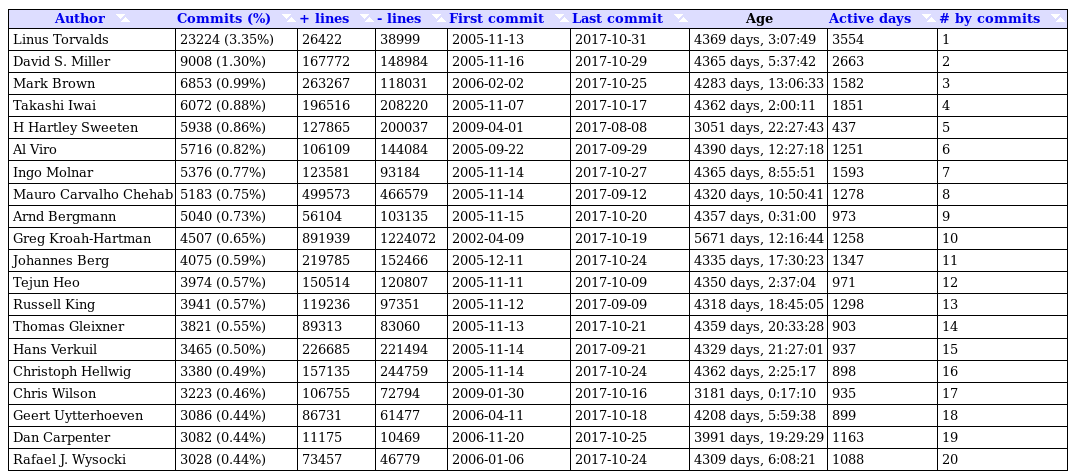
\includegraphics[scale=0.40]{images/top_20_of_linux_authors.png}
	\caption{Top 20 Linux Kernel Autoren}
	\label{top20}
\end{figure}

Diese Statistiken wurden entweder mit gitstats\cite{link:gitstats} oder standard
Git Befehlen ermittelt. So lassen sich z.B. unter Linux, die durchgeführten
Merges von Linus Torvalds mit folgendem Befehl ermitteln:

\lstinputlisting[
  label=lst:allmerges,
  caption={Ermitteln von Merges pro Autor},
]{listings/all_merges.lst}

Statistiken, wie o.a. sind aber nicht unbedingt als Qualitätsmaßstab geeignet um
Rückschlüsse auf die Effizienz einzelner Personen zu ziehen. Wie in Kapitel
\ref{sec:collaboration} beschrieben, sollten diese Informationen aber trotzdem
allen Beteiligten zur Verfügung gestellt werden.  So wird nach Jez Humble und
David Farley in \cite[S.~138]{cd} eine Messung der geschriebenen Zeilen
Quellcode am Tag wahrscheinlich eher dazu führen, dass Entwickler kürzere Zeilen
Quellcode als effizientere schreiben. Die gemessene Anzahl an Commits führt hingegen
evtl. dazu, dass Änderungen pro Commit kleiner werden und dadurch besser
nachvollziehbar. So schreiben Jeniffer Davis und Katherine Daniels in
\cite[S.~179]{effdo} zu der Anzahl geschriebener Zeilen Quellcode:
\begin{center}
\textit{\glqq{}Lines of code is not an accurare measure of value. There are
different types of developers, some that refactor hundreds of confusing lines
into tens of lines of simple-to-read abstractions that can be build upon by
others in the team.\grqq{}}
\end{center}

Eine genauere Betrachtung von Abbildung \ref{top20} bekräftigt diese Aussage.
Linus Torvalds führt zwar die Liste der meisten Commits an, hat aber weder die
meisten Zeilen hinzugefügt noch entfernt. Greg Kroah-Hartman hingegen liegt
nach der Anzahl der Commits auf Platz 10 und hat mit stattlichen 1.224.072
hinzugefügten und 891.939 entfernten Zeilen, wie auch die meisten anderen aus
der Liste, weit mehr Zeilen zum Kernel beigetragen, als Linus Torvalds selbst.
Die Betrachtung der reinen Zahlen reicht also nicht aus, um eine repräsentative
Einschätzung einzelner Personen zu erhalten.

Es können verschiedenste Statistiken über ein Projekt bzw. Repository erhoben
werden, die geeignet sind ein, vollständigeres Bild über die Aktivitäten
innerhalb des Projektes zu bilden. Beispielsweise könnten das nach Jez Humble
und David Farley in \cite[S.~138]{cd}folgende sein:

\begin{itemize}
\item Testabdeckung,
\item Anzahl der Fehler,
\item Anzahl der \glspl{commit},
\item Anzahl der fehlgeschlagenen/erfolgreichen Versuche, die Software zu erstellen,
\item Metriken über den Quellcode (Zyklen, Duplikate o.a.),
\end{itemize}
